\documentclass{article}
\usepackage{tikz}
\begin{document}

  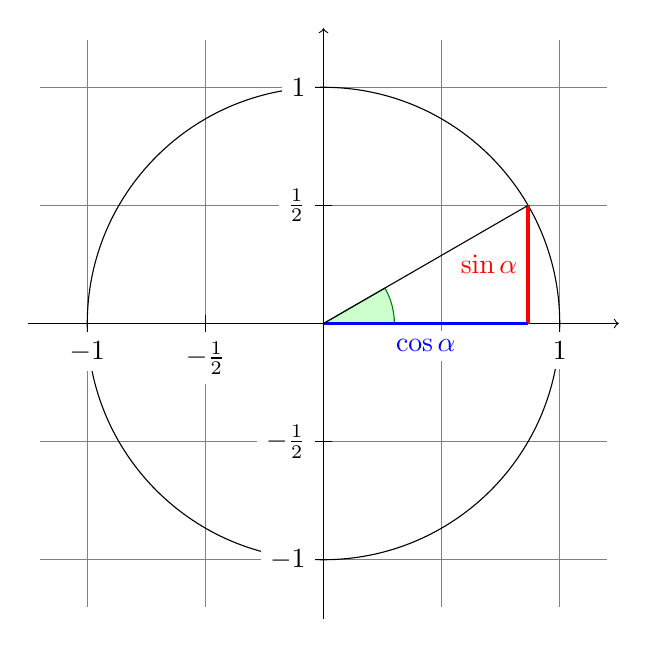
\begin{tikzpicture}[scale=3]
    \draw[step=.5cm, gray, very thin] (-1.2,-1.2) grid (1.2,1.2); 
    \filldraw[fill=green!20,draw=green!50!black] (0,0) -- (3mm,0mm) arc (0:30:3mm) -- cycle; 
    \draw[->] (-1.25,0) -- (1.25,0) coordinate (x axis);
    \draw[->] (0,-1.25) -- (0,1.25) coordinate (y axis);
    \draw (0,0) circle (1cm);
    \draw[very thick,red] (30:1cm) -- node[left,fill=white] {$\sin \alpha$} (30:1cm |- x axis);
    \draw[very thick,blue] (30:1cm |- x axis) -- node[below=2pt,fill=white] {$\cos \alpha$} (0,0);
    \draw (0,0) -- (30:1cm);
    \foreach \x/\xtext in {-1, -0.5/-\frac{1}{2}, 1} 
      \draw (\x cm,1pt) -- (\x cm,-1pt) node[anchor=north,fill=white] {$\xtext$};
    \foreach \y/\ytext in {-1, -0.5/-\frac{1}{2}, 0.5/\frac{1}{2}, 1} 
      \draw (1pt,\y cm) -- (-1pt,\y cm) node[anchor=east,fill=white] {$\ytext$};
  \end{tikzpicture}

\end{document}

